\documentclass[a4paper]{article}

\def\npart {SUROP}
\def\nterm {Summer 2016}
\def\ncourse {Shadow tomography}

% Imports

\usepackage[pdftex,colorlinks=true]{hyperref}
\usepackage[T1]{fontenc}
\usepackage{lipsum}
\usepackage{amsfonts}
\usepackage{amsmath}
\usepackage{amssymb}
\usepackage{amsthm}
\usepackage{booktabs}
\usepackage{caption}
\usepackage{enumitem}
\usepackage{graphicx}
\usepackage{mathtools}
\usepackage{microtype}
\usepackage{multirow}
\usepackage{pdfpages}
\usepackage{siunitx}
\usepackage{tabularx}
\usepackage{tikz}
\usepackage{todo}
\usepackage{fancyhdr}
\usepackage{ifthen}
\usepackage[normalem]{ulem}
\usepackage{pdflscape}
\usepackage{lmodern}
\usepackage{listings}
\usepackage{floatrow}%

\pagestyle{fancyplain}
\lhead{\emph{\nouppercase{\leftmark}}}
\ifx \nextra \undefined 
  \rhead{\ifthenelse{\value{page}=1}{}{\npart\ \ncourse}}
\else
  \rhead{\ifthenelse{\value{page}=1}{}{\npart\ \ncourse\ (\nextra)}}
\fi
\usetikzlibrary{arrows}
\usetikzlibrary{decorations.markings}
\usetikzlibrary{positioning}
\usetikzlibrary{calc}

% Theorems
\theoremstyle{definition}
\newtheorem*{aim}{Aim}
\newtheorem*{axiom}{Axiom}
\newtheorem*{claim}{Claim}
\newtheorem*{cor}{Corollary}
\newtheorem*{defi}{Definition}
\newtheorem*{eg}{Example}
\newtheorem*{fact}{Fact}
\newtheorem*{law}{Law}
\newtheorem*{lemma}{Lemma}
\newtheorem*{notation}{Notation}
\newtheorem*{prop}{Proposition}
\newtheorem*{thm}{Theorem}

% Latex constructs
\newcommand{\mb}[1]{\mathbf{#1}}
\newcommand{\note}{\vspace{3pt}\noindent \emph{Note}:\;}
\newcommand{\argmin}{\operatornamewithlimits{argmin}}

\renewcommand{\labelitemi}{--}
\renewcommand{\labelitemii}{$\circ$}
\renewcommand{\labelenumi}{(\roman{*})}

\let\stdpart\part
\renewcommand\part{\newpage\stdpart}

\let\stdsection\section
\renewcommand\section{\stdsection}

\newcommand{\img}[2][]{\begin{center}\centering\includegraphics[#1]{images/#2.pdf}\end{center}}

% Strike through
\def\st{\bgroup \ULdepth=-.55ex \ULset}

% Maths symbols
\newcommand{\bra}{\langle}
\newcommand{\ket}{\rangle}

\newcommand{\N}{\mathbb{N}}
\newcommand{\Z}{\mathbb{Z}}
\newcommand{\Q}{\mathbb{Q}}
\newcommand{\R}{\mathbb{R}}
\newcommand{\C}{\mathbb{C}}
\newcommand{\Prob}{\mathbb{P}}
\renewcommand{\P}{\mathbb{P}}
\newcommand{\E}{\mathbb{E}}
\newcommand{\F}{\mathbb{F}}
\newcommand{\cU}{\mathcal{U}}

\DeclareMathOperator{\im}{Im}
\DeclareMathOperator{\re}{Re}

\DeclareMathOperator{\tr}{tr}
\DeclareMathOperator{\diag}{diag}
\DeclareMathOperator{\rank}{rank}
\DeclareMathOperator{\card}{card}
\DeclareMathOperator{\spn}{span}

\DeclareMathOperator{\erf}{erf}
\DeclareMathOperator{\erfc}{erfc}

\DeclareMathOperator{\ord}{ord}
\DeclareMathOperator{\Sym}{Sym}

\DeclareMathOperator{\sgn}{sgn}
\DeclareMathOperator{\orb}{orb}
\DeclareMathOperator{\stab}{stab}
\DeclareMathOperator{\ccl}{ccl}

\DeclareMathOperator{\lcm}{lcm}
\DeclareMathOperator{\hcf}{hcf}

\DeclareMathOperator{\Int}{Int}
\DeclareMathOperator{\id}{id}

\DeclareMathOperator{\betaD}{beta}
\DeclareMathOperator{\gammaD}{gamma}
\DeclareMathOperator{\Poisson}{Poisson}
\DeclareMathOperator{\binomial}{binomial}
\DeclareMathOperator{\multinomial}{multinomial}
\DeclareMathOperator{\Bernoulli}{Bernoulli}
\DeclareMathOperator{\like}{like}

\DeclareMathOperator{\var}{var}
\DeclareMathOperator{\cov}{cov}
\DeclareMathOperator{\bias}{bias}
\DeclareMathOperator{\mse}{mse}
\DeclareMathOperator{\corr}{corr}

\DeclareMathOperator{\otp}{otp}
\DeclareMathOperator{\dom}{dom}

\newcommand{\GL}{\mathrm{GL}}
\newcommand{\SL}{\mathrm{SL}}
\newcommand{\Or}{\mathrm{O}}
\newcommand{\SO}{\mathrm{SO}}
\newcommand{\U}{\mathrm{U}}
\newcommand{\SU}{\mathrm{SU}}

\renewcommand{\d}{\mathrm{d}}

\tikzset{->/.style = {decoration={markings,
                                  mark=at position 1 with {\arrow[scale=2]{latex'}}},
                      postaction={decorate}}}
\tikzset{<-/.style = {decoration={markings,
                                  mark=at position 0 with {\arrowreversed[scale=2]{latex'}}},
                      postaction={decorate}}}
\tikzset{<->/.style = {decoration={markings,
                                   mark=at position 0 with {\arrowreversed[scale=2]{latex'}},
                                   mark=at position 1 with {\arrow[scale=2]{latex'}}},
                       postaction={decorate}}}
\tikzset{->-/.style = {decoration={markings,
                                   mark=at position #1 with {\arrow[scale=2]{latex'}}},
                       postaction={decorate}}}
\tikzset{-<-/.style = {decoration={markings,
                                   mark=at position #1 with {\arrowreversed[scale=2]{latex'}}},
                       postaction={decorate}}}

\tikzset{circ/.style = {fill, circle, inner sep = 0, minimum size = 3}}


\begin{document}
\title{
    SUROP \\ Progress report
}
\title{Summer Undergraduate Research Opportunities}
\date{July, 2016}
\author{Emile Okada \\ University of Cambridge}
\maketitle

\newpage

\setcounter{section}{0}
\section{Week 1}
\subsection{Reading}
I started the week reading Chapter 1 section 2 of Charles L. Epstein's "Introduction to the Mathematics of Medical Imaging".
It covered how to reconstuct a 2D convex object from the shadows of an object. 
If $h(\theta)$ is the shadow function as described in the book (essentially the distance of the support line in direction $(-\sin(\theta),\cos(\theta))$ from the origin), then the convex hull can be parameterized by

\begin{equation}
    (x(\theta),y(\theta)) = h(\theta)\cdot(\cos(\theta),\sin(\theta))+h'(\theta)\cdot(-\sin(\theta),\cos(\theta)).
\end{equation}

We can extend this idea to 3D by considering slices of the object. 
Fix some vector {\bfseries v} and then consider the collection of planes perpendicular to {\bfseries v}. 
In each of the planes one can use the 2D method to construct a 2D convex hull of the intersection of the object with the plane. 
Stringing all these 2D slices together then gives a rough reconstruction of the 3D object from its shadows.

I also spent some time reading up on the TV transform and scale spaces, to get a rough idea of which project I'd like to do. 
I ended up going with the tomography project, but spend roughly 1.5 days doing reading for the other project.

\subsubsection{Remaining tasks}
The above method only allows for 'slicewise convex' reconstructions. While better than convex, this doesn't ustilize all the data available from the shadows e.g. see the rabit ears below. We know the two ears are two separate 'blobs' and we can tell this from the shadow, but this information is nonetheless lost in the reconstruction. I will try to find ways on how to improve on this (so that e.g. if we scan a human we can see two legs rather than one large blob).

\subsection{Coding}
On Thursday I started coding. 
To have some examples to work with I used the Wolfram Mathematica ExampleData function to obtain a 3D model of a rabit.

\begin{figure}[H]
  \centering
    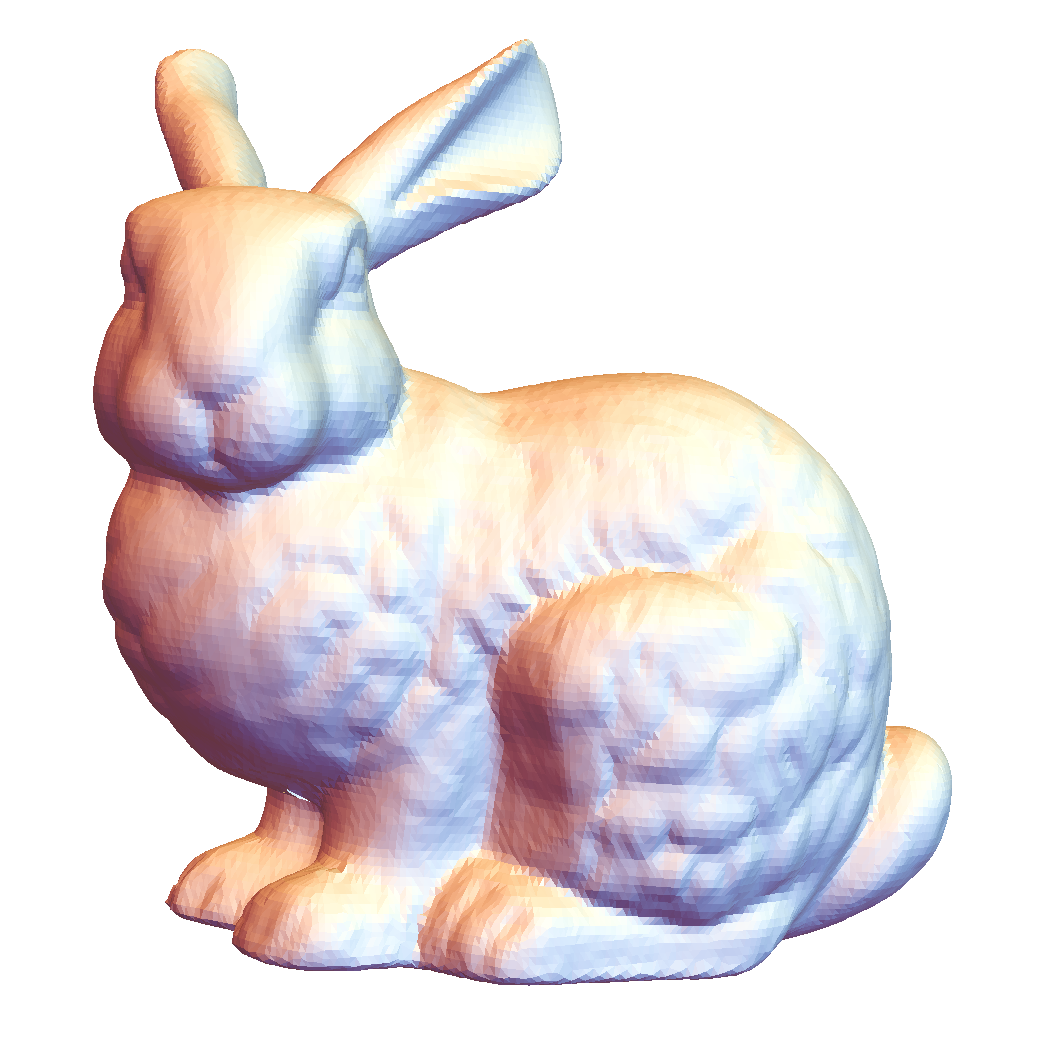
\includegraphics[width=0.4\textwidth]{figures/3D_rabit.png}
    \caption{3D model of a rabit from Mathematica ExampleData.}
  \label{fig:f2}
\end{figure}

I then took its orthogonal projection and binarized the image to obtain shadows of the rabit from 10 different angles.

\begin{figure}[H]
    \begin{floatrow}
        \ffigbox{
\includegraphics[scale = 0.5]{figures/space1.jpg}}{\caption{Shadow of rabit with $\theta=0$.}\label{fig:err1}}
        \ffigbox{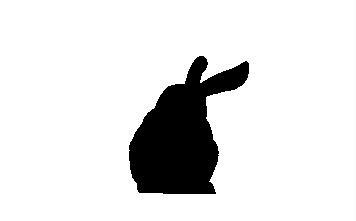
\includegraphics[scale = 0.5]{figures/space5.jpg}}{\caption{Shadow of rabit with $\theta=\pi/2$.}\label{fig:err2}}
    \end{floatrow}
\end{figure}

I then finished writing the code for reconstructing the object from its shadows in python (see page \pageref{alg:shadow} or my \href{https://github.com/emileokada/image3d}{github}) on Friday.

\begin{figure}[H]
  \centering
    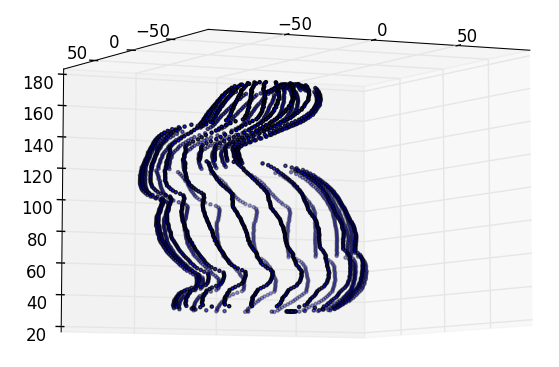
\includegraphics[width=0.7\textwidth]{figures/rabit.png}
    \caption{Reconstruction of the rabit using the script on page \pageref{alg:shadow}.}
  \label{fig:f2}
\end{figure}

\subsubsection{Challenges}
I had some problems originally with taking the derivative of the shadow function since the input was a bit noisy.
To fix this problem I convolved the data with a discrete gaussian (binomial distribution) to smooth out the noise.
This worked well with the example data. 
However, it remains to see whether it will work well enough for the actual real life pictures which will probably be a lot more noisy.

\subsubsection{Remaining tasks}
There are currently a lot more data points than I need. At the moment I'm calculating the shadow function fow each row of the image matrix.
This results in a lot of points which causes the rendering to take some time.
I can probably get away with a lot fewer points in the z direction.
I also plan on adding a polygonal mesh so it looks a bit nicer.
Lastly, I should probably also do some smoothing in the z direction to fix the sudden cutoffs that tend to occur when the variations in the 3D object are smaller than the 'resolution' in the z-direction.

\begin{figure}[H]
  \centering
    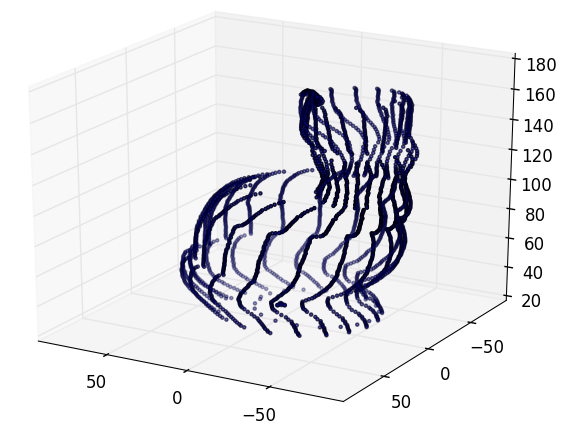
\includegraphics[width=0.7\textwidth]{figures/ear_and_back_cutoff.png}
    \caption{Cutoff of rabits ears. Can probably be fixed by smoothing the data in the z direction.}
  \label{fig:f2}
\end{figure}

\subsection{Building}
I haven't begun building yet, but I now have a rough idea of the the set should look like. 
At the moment I'm thinking of creating a simple turn table (rotating platform) on which a person stands. I'll then place some bright lights in front for them and a big white sheet of paper behind on which to shine their shadow. 
A camera is then placed behind the paper to capture the shadows.

\subsubsection{Remaining tasks}
I'll create a proper design this week and make a basic prototype on a smaller scale hopefully by next week.

\section{Week 2}
\subsection{Reading}
This week I had a chat with Martin and Matthias on how to resolve objects like rabit ears (i.e. disjoint unions of convex objects).
They suggested a 'back projection' method that is a generalization (or in some sense a generalization of the 'dual') of the method from week 1.
The methods can be thought of as follows: imagine standing inside a circle with walls around. 
Every, say, $\pi/8$ radians there is a light source that creates a shadow diagonally opposite.
Now extend each shadow out of the wall to the opposite side, to create 'cylinders' with cross sections with the shape of the shadow.
We then intersect these cylinders to get the reconstruction.
In some sense this method utilizes all the information available and can distinguish between legs, rabit ears and other disjoint unions of convex blobs. 
We also don't need to differentiate anything with this method which is always nice.

\subsubsection{Remaining tasks}
Read up on TV smoothing for 3D surfaces to make smoother reconstructions.

\subsection{Coding}
Before I implemented the new method I added a polygonal mesh to the original method.

\begin{figure}[H]
  \centering
    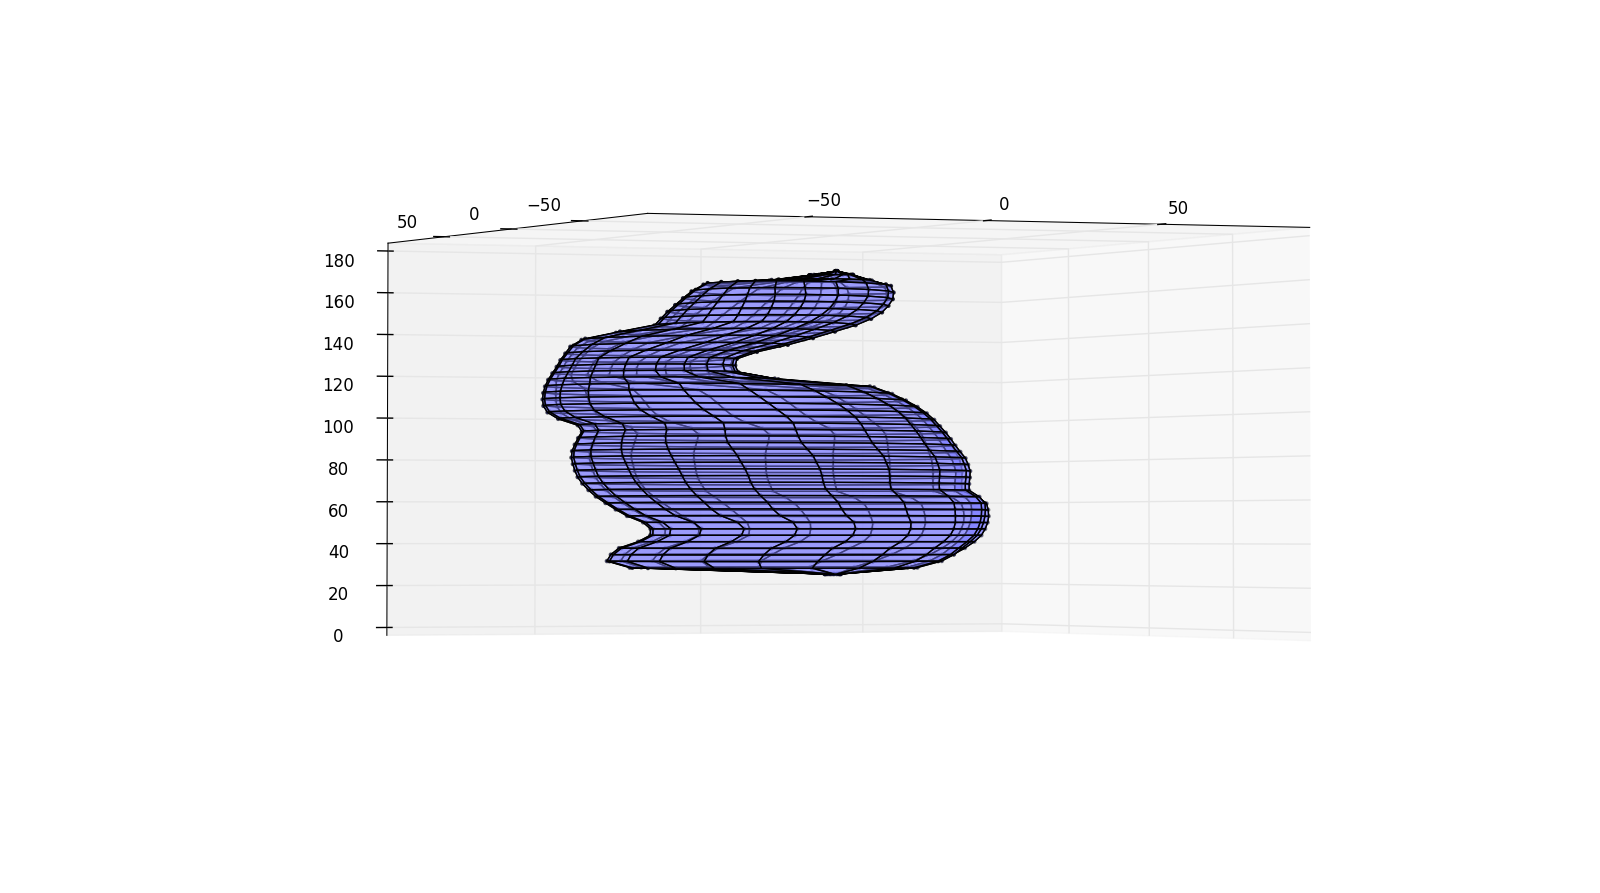
\includegraphics[width=0.7\textwidth]{figures/polygonal_mesh.png}
    \caption{Original reconstruction with polygonal mesh added.}
  \label{fig:f2}
\end{figure}

I also implemented the new method.
It works by reducing it to the 2D version of the problem and doing the reconstruction by slices like the previous method.
It is slightly more computationally expensive (the 'cyclinders' are represented in arrays and the intersection is done by pointwise multiplication).
However, there results are a lot better.

\begin{figure}[H]
  \centering
    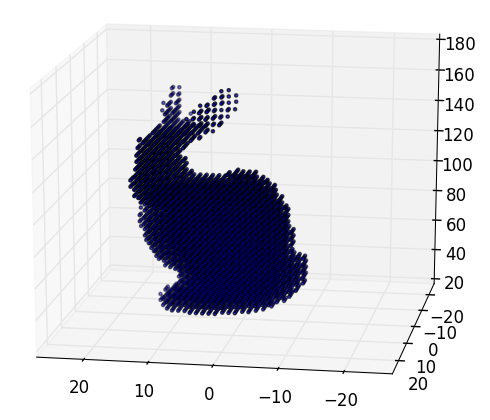
\includegraphics[width=0.7\textwidth]{figures/rabit_ears_3.png}
    \caption{Reconstruciton of rabit with two disjoint ears.}
  \label{fig:f2}
\end{figure}

I also implemented a method that only displays the boundary of the reconstructions by taking the morphological perimeter of each slice.

\begin{figure}[H]
  \centering
    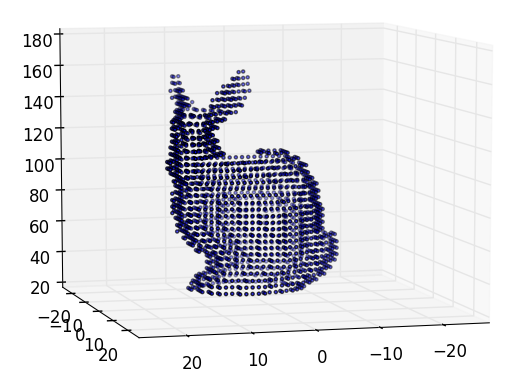
\includegraphics[width=0.7\textwidth]{figures/rabit_ears_4.png}
    \caption{Boundary of rabit reconstruciton.}
  \label{fig:f2}
\end{figure}

\subsubsection{Remaining tasks}
It would be good to add a mesh to this method as well and maybe get some lighting to make it look more realistic.
Also need to implement TV method, but will probably wait to do that until I have something that works first.

\subsection{Building}
I've done some reseach on turntables for humans. I've found quite a few DIY turntables that are cheap and relatively straightforward to make (see \href{http://hackaday.com/2015/05/23/3d-scanning-rig-and-diy-turntable/}{this}, \href{http://www.thingiverse.com/thing:729923}{this} and \href{http://hackaday.com/2016/02/25/hacked-turntable-rotates-humans-for-3d-scanning/}{this}).
I also looked for some ready made ones, but the ones I found were either too expensive (€650) or made for mannequins so can't take the full load of a human.
It seems like the best option would be to make my own. I'll contact the engineering department to ask if there is any way I could use some of their tools (possibly under the supervision of an engineering friend) to make the turntable myself.
I've also looked at lighting and it seems quite cheap so shouldn't be a problem.
Hopefully I'll start ordering the equipment this week.

\section{Week 3}
\subsection{Reading}
This week I read up on ROF denoising and the TV transform. In particular I read the Chambolle \& Pock paper.
I then extended the ROF denoising algorithm to 3D 'images' in the obvious way.

\subsection{Coding}
In preparation for the 3D version of the TV denoising algorithm I implemented the 2D version as outlined in the paper.

\begin{figure}[H]
  \centering
    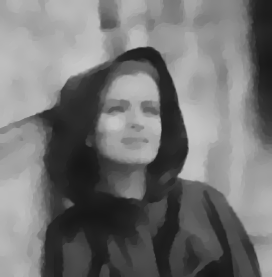
\includegraphics[width=0.4\textwidth]{figures/denoised.png}
    \caption{Look, less noise! (with very few iterations since python is slow...)}
  \label{fig:f2}
\end{figure}

I then implemented the 3D version. Here is a sample output:

\begin{figure}[H]
  \centering
    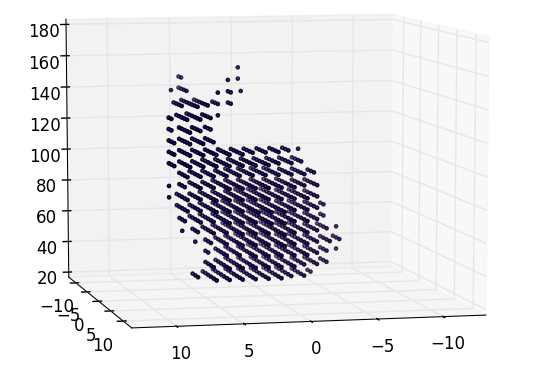
\includegraphics[width=0.7\textwidth]{figures/smooth_rabit.png}
    \caption{Denoised rabit. It doesn't look very different however since the input data didn't have much noise to start with. This is good!}
  \label{fig:f2}
\end{figure}


\subsubsection{Remaining tasks}
I should probably make the rabit look solid rather than a cloud of dots. I should also test the algorithm on some noisy data as well.
Maybe I can add in some facny lighting and fun statistics about water content and whatnot (for the purpose of the science fair).
I think I'll also reimplement the code in Matlab since python is super slow.

\subsection{Building}
I set up a meeting with the dyson center in the engineering department this week. We might be able to use their spaces to construct the scanner.
We discussed how to make the turntable in particular. One of the designs we looked at however seemed somewhat difficult to make and would probably require us to hire the workshop to make it. 
I'll thus look more into the simpler looking turntable. 

\subsubsection{Remaining tasks}
I need to make some accurate drawings for the turntable.
I'll need exact measurements etc. and also I need to find the parts I need. Then I can make a cost estimate and then meet with the people in the engineering department again to discuss feasiblity.

\section{Week 4}

My parents came to visit over the weekend + Monday and left on Tuesday so didn't get as much done as I'd like. I also spent Thursday + Friday preparing the presentation for the group meeting.

\subsection{Building}
On Tuesday I visited the Dyson Center to ask about the designs and using their space.
One of the designs for the turntable that I had found was probably a bit beyond my technical skills so I decided to go for the simpler design.
While there they kindly explained the key parts of the design and what a bearing was.
They also said they had to double check that it was ok that we used space in the Dyson Center since we were from the maths department. Hopefully they will get back to us soon.

I've also looked more closely at what I need to do buildingwise and started looking up parts. A rough upper bound on the cost of the turn table is \pounds 100. This includes the cost of plywood, wood glue, bearings, motor, and the computer components (bluetooth component and arduino nano to control the motor remotely). 
Note that this is an upper bound and can probably be brought down maybe \pounds 30-\pounds 40.

The shadow screen will probably be quite a bit cheaper. A 2m PVC pipe costs roughly \pounds 3. Trow in the cost of some joints and the fabric (this is the most expensive part, maybe \pounds 25, but I'll look for some cheaper alternatives) and the total can be roughly bounded above by \pounds 50.

The last remaining part is the light. I noticed that the light from a projector is very strong and might be able to do the trick. If not, I found some outdoor lights that cost \pounds 8, so I just need something to mount them on.

\subsection{Remaining tasks}
This week I need to start ordering the parts. Then hopefully I can start building something next week.

\section{Week 5}
This week I was helping out with a maths summer school in the mornings (9am-11am) since I'm mostly just waiting for parts to arrive.

\subsection{Reading}
This week Martin explained to me an alternate way to perform the smoothing on the 3D reconstruction.

The idea is to solve
\begin{equation}
    \hat u = \argmin_u \{\text{TV}(u) \text{ s.t. } SR(u)=0, u\in[0,1]\}
\end{equation}
where $R$ is the discrete Radon transform and S is a subsampling operator which depends on the input image (it ensures that the Radon tranform of $u$ stays 0 at the same places as for the inital images).

To solve this problem we can use the Chambolle Pock framework by letting 
\begin{align*}
    F(y_1,y_2) &= \chi_{\cdot = 0}(y_1)+\|\|y_2\|_2\|_1 \\
    G(x) &= \chi_{[0,1]}(x) \\
    K &= (SR,\nabla)^T
\end{align*}

\subsubsection{Remaining tasks}
I'll need to actually implement this. Doesn't seem like too much work, but will wait till I've actually made the 3D-scanning device first.

Anothering that I need to do is find a robust way to generate a polygonal mesh of the reconstructed object. I can't seem to find an easy way to do this.

\subsection{Building}
Over the past week I begun ordering all the parts we need.
The main difficulty has been in obtaining furniture grade PVC fittings in the UK.
The DYI market is large in the US, but quite small in the UK. 
The only seemingly decent supplier in the UK however is currently not in operation due to a wedding of some sorts (?) (it is a very small company).
I we've thus resorted to ordering the fittings from Germany, and the pipes from the UK.

Otherwise, we now have the fabric, wood glue, Lazy Susan bearings, extension cords, webcam, motor and printer.

It remains to order some of the electronic circuit components, plywood and possibly a usb extension cable.

I also went to the Dyson center to get some advice. Here are scans of the sketches that Dr. Roebuck made while explaining how to make the electric ciruit and where to get plywood.
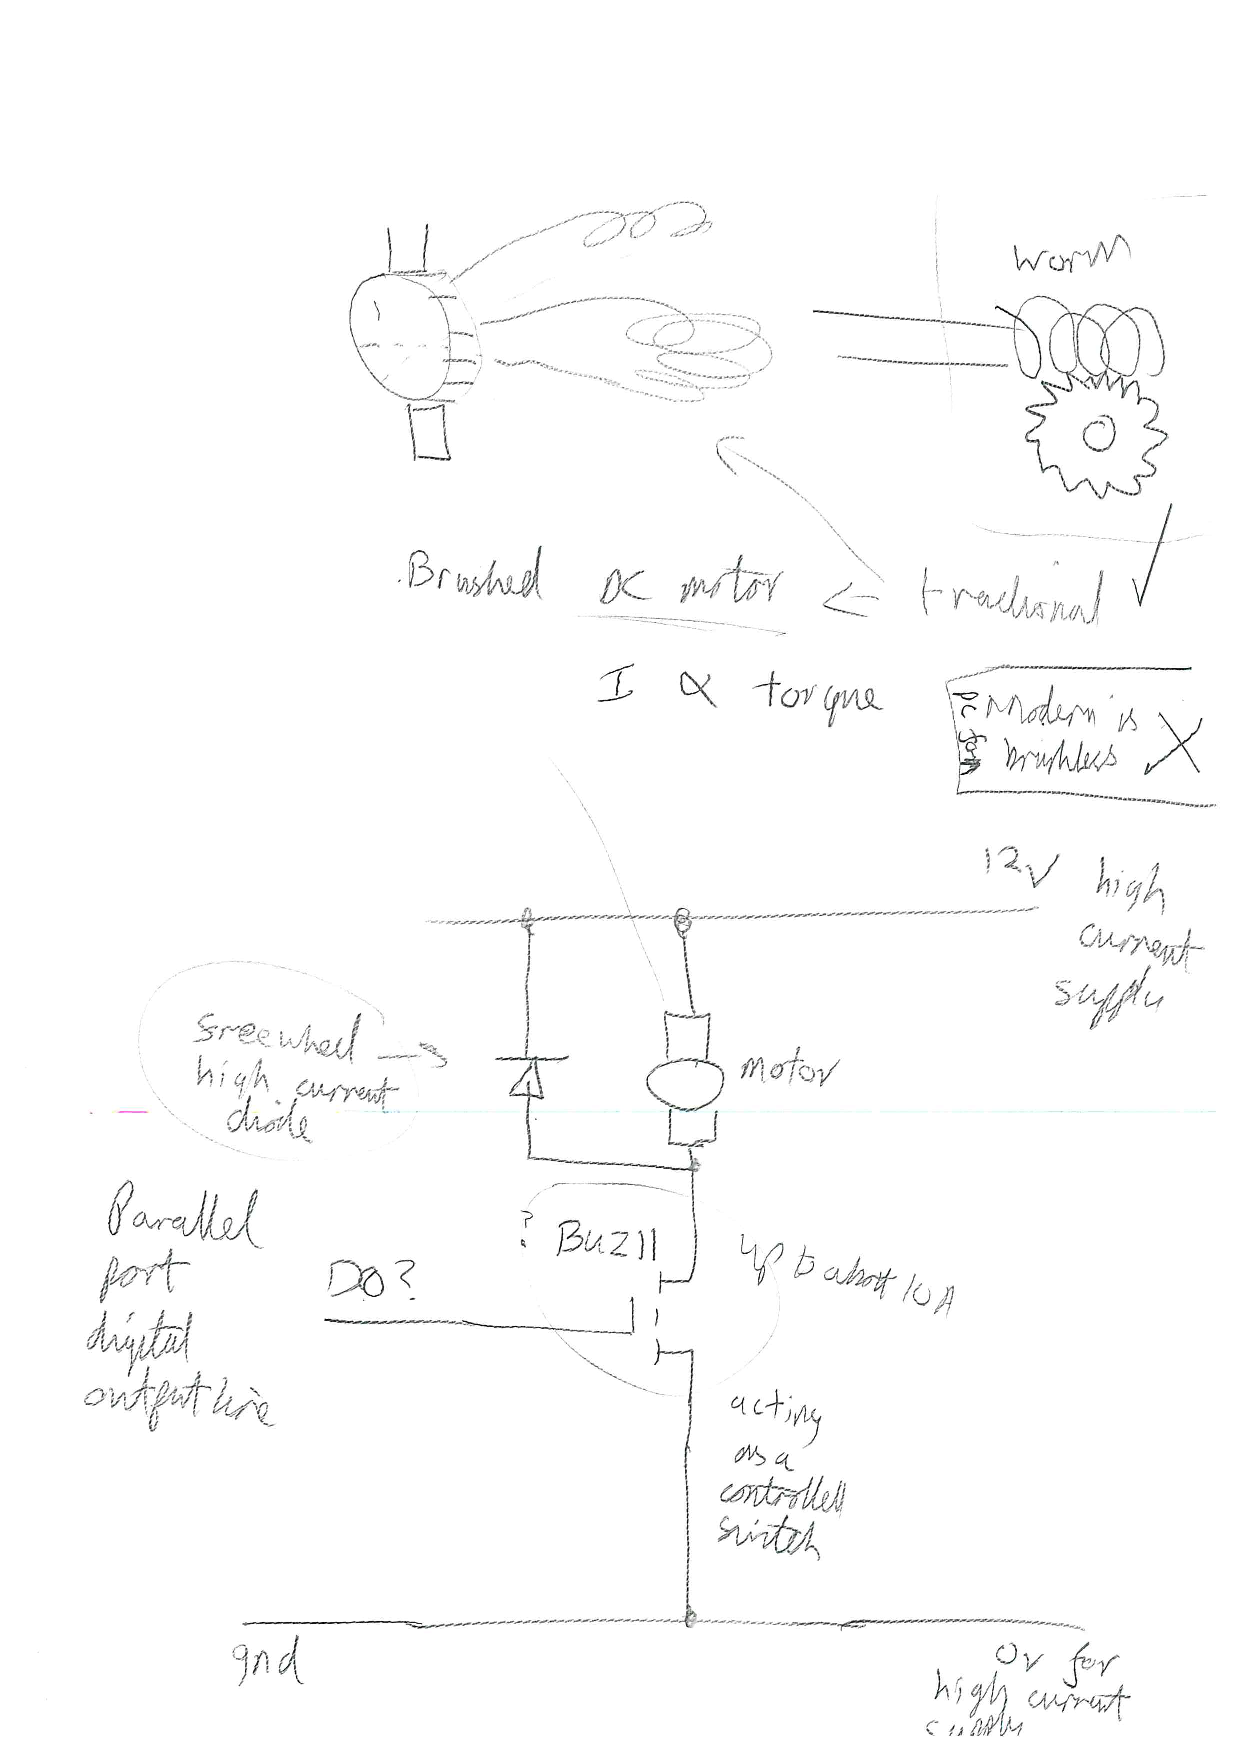
\includepdf[pages={1,2}]{figures/drawings.pdf}

\section{Week 6}

\subsection{Reading}
This week I've read up a bit on electronic circuits.
After talking to Dr. Roebuck, I got some advice on what sort of components I'd need to control the motor using a computer.
As such I've read up on MOSFETs, parallel ports and microswitches.
The parallel port allows me to connect the circuit to the computer, while the MOSFET acts as a switch to turn the motor on an off.
Lastly, the microswitch can help keep track of how many degrees the turntable has tunred by counting the numer of teeth that have passed by.

\subsubsection{Remaining tasks}
I'll need to find a way to undo the warping caused by the wide angle webcam.

\subsection{Coding}
After talking to Matthias, it turns out matlab has an 'isosurface' function which allows me to create a surface around the reconstructed object and add lighting and shadows. As such I've been migrating my python code to matlab.
The other reason I'm doing this is because matlab seems to be quite a bit quicker with dealing with large array's of the type I'm working with.
I've migrated rougly half of the code now and intend to finish by the end of this week.

\subsection{Building}
The PVC pipes have now arrived and we're only waiting for the fittings from Germany now.
It seems like the muslin cloth for my backdrop is taking longer than anticipated to arrive so I might have to send an email to enquire.
The plywood has also been ordered so I should be able to start cutting it by midweek.
The motor is also here now, so I only need to order the remaining electronic components.
All that remains is dealing with the lighting. 
I've emailed a friend who is an engineer at a lighting company in Cambridge to ask for his advice. 
He had previously mentioned that we might be able to inherit some spare lighting or at the very least get some tips on what kind of strength we need to get a decent shadow in a standardly illuminated room.

\subsubsection{Changes}
I've made some modifications to the design of the shadow screen.
With the new wide angled webcam, I can place the webcam roughly 1m away from the screen. As such I intend to adjoin an additional structure to the screen to ensure that the webcam stays at a fixed position relative to the screen.
This way I can also hopefully correct for the distortions caused by the wide angle lens since I know precisely the distance between the webcam and the shadow screen.

\begin{figure}[H]
  \centering
    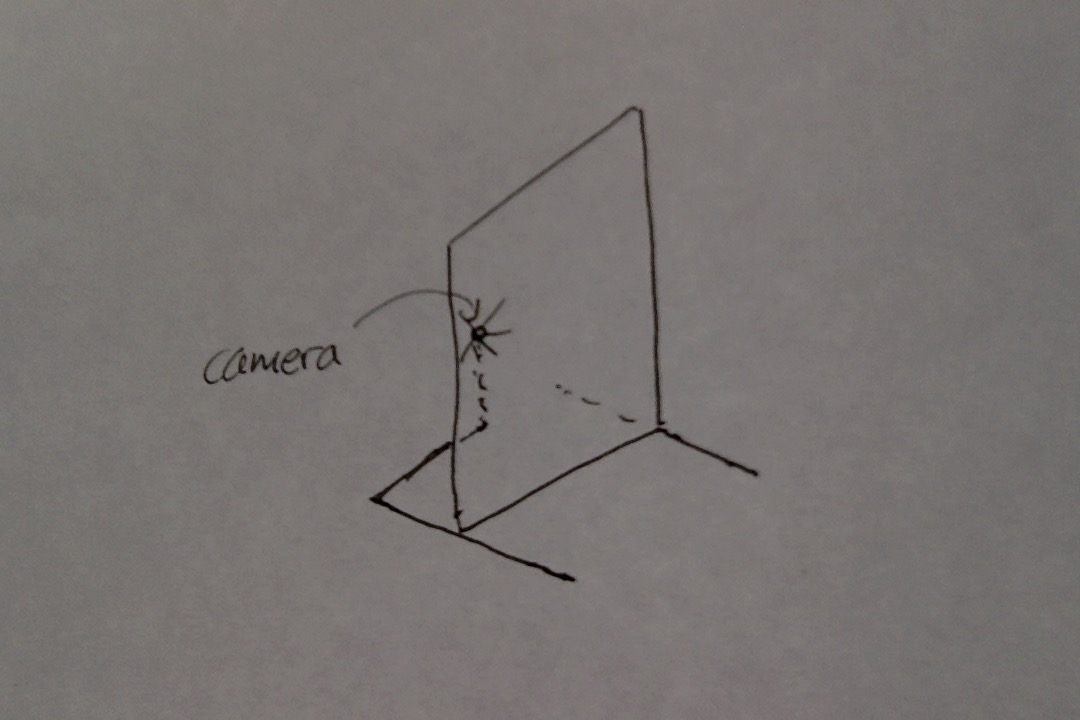
\includegraphics[width=0.4\textwidth]{figures/new_setup.jpg}
    \caption{Mounting of the webcam.}
  \label{fig:f2}
\end{figure}

\subsubsection{Remaining tasks}
Other than obviously assembling the setup, I need to determine a proper power supply. 
The engineering department has kindly allowed me to borrow one of their variable power supplies so that I can determine what kind of current I need.
Thus once the turntable is functional and tested I can buy a fixed current power supply.

\section{Week 7}

\subsection{Coding}
This week I finished rewriting all the code in Matlab.
I also added some new functionality.
The program now creates a surface mesh and adds lighting to the reconstruction.

\begin{figure}[H]
  \centering
    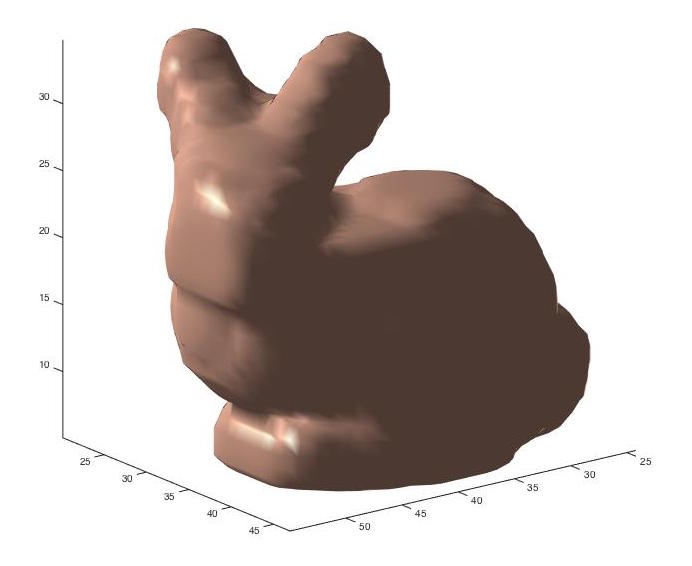
\includegraphics[width=0.7\textwidth]{figures/rabit_surface.jpg}
    \caption{Reconstructed rabit with surface mesh and lighting.}
  \label{fig:f2}
\end{figure}

A higher resolution can be obtainted by lowering the 'xy\_scaling' parameter in the 'recon' class, but the tradeoff is that it becomes quite a bit slower.

\subsubsection{Remaining tasks}
Create an interface which people at the science fair can use.
In other words, a start button to rotate the person and then an interface which allows them to view the object from different angles.

\subsection{Building}
The frame of the shadow screen was completed this week.
The pvc pipes were cut into two 2m pieces, two 1.5m pieces, one 1m piece, one 0.75m piece and four 0.5m pieces.
Assembly takes roughly 1min so is very convenient. The finished frame looks like

\begin{figure}[H]
  \centering
    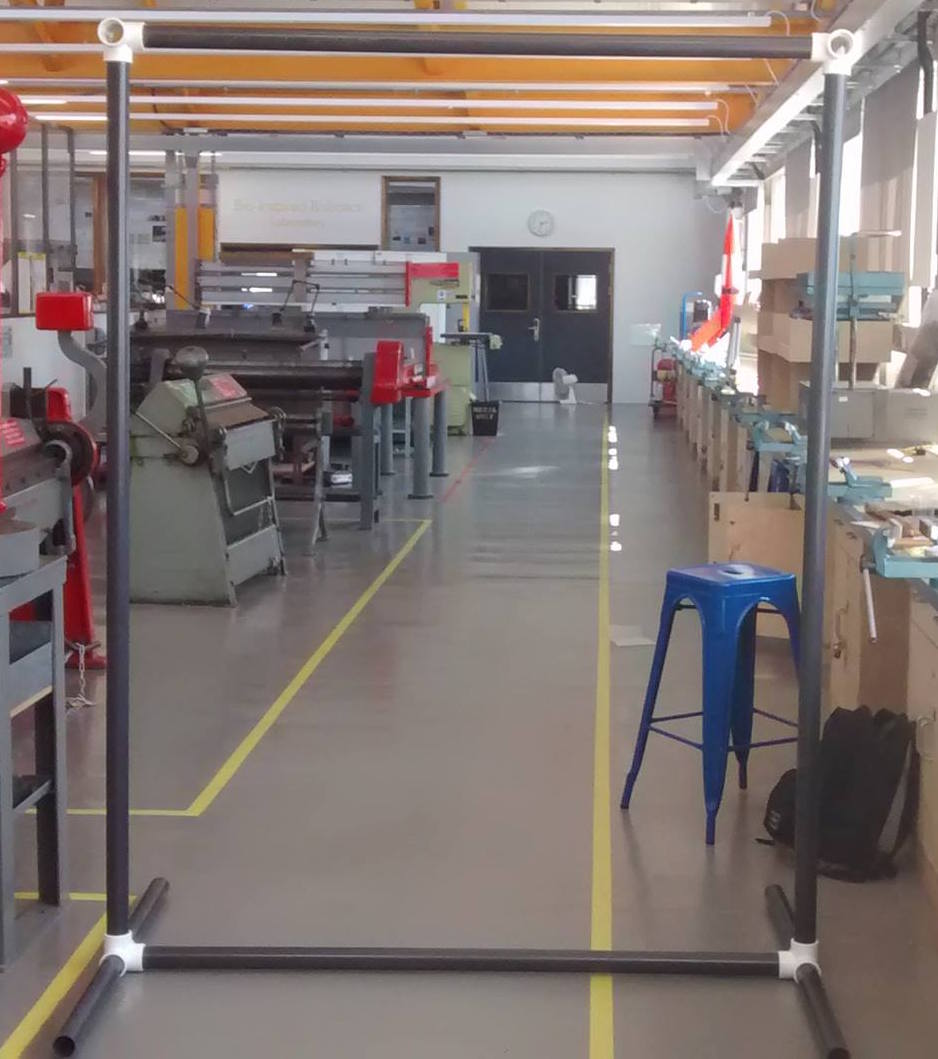
\includegraphics[width=0.7\textwidth]{figures/skeleton.jpg}
    \caption{Frame of shadow screen.}
  \label{fig:f2}
\end{figure}

The fabric also arrived and came in one 2m by 1.5m peice.
To attach the fabric to the frame I decided to sew on elastic cloth as 'handles'. 

One early problem that I found was that the fabric was letting too much light in.
While the shadow was nice and clear on the side that was illuminated, from the back it got washed out by the weaker ambient lighting.

\begin{figure}[H]
  \centering
    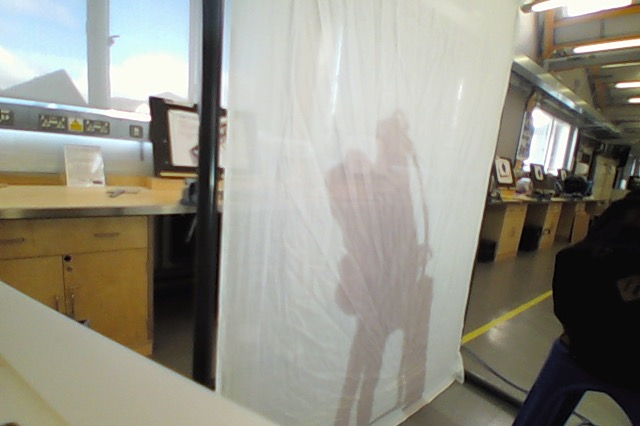
\includegraphics[width=0.7\textwidth]{figures/clear_shadow.jpg}
    \caption{The shadow from the front view is nice and clear...}
  \label{fig:f2}
\end{figure}

\begin{figure}[H]
  \centering
    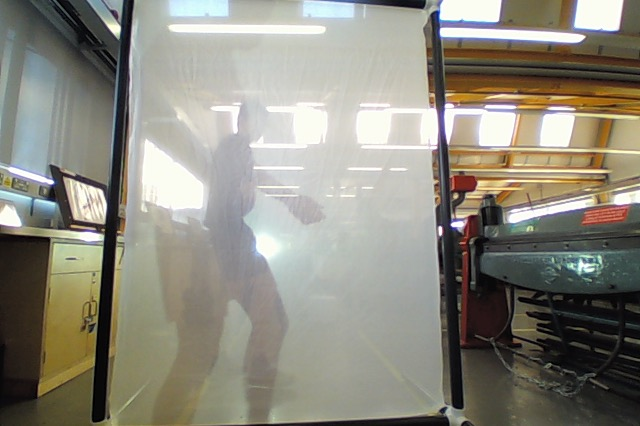
\includegraphics[width=0.7\textwidth]{figures/rear_shadow.jpg}
    \caption{... however the current fabric is too transparent so the camera picks up the ambient background lighting as well as the actual object.}
  \label{fig:f2}
\end{figure}

To try to fix the problem I tried folding the fabric to see if increasing the thickness helped improve clarity.

\begin{figure}[H]
  \centering
    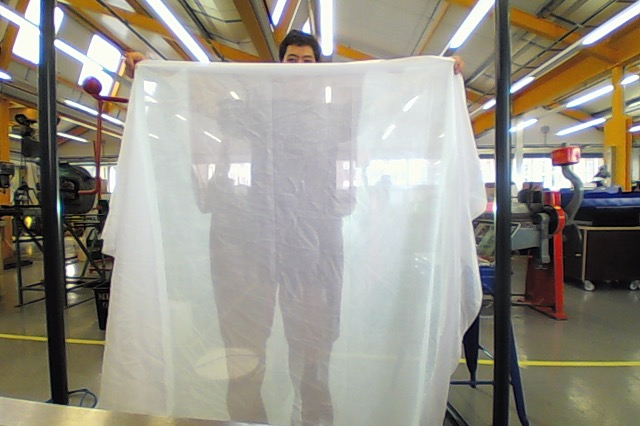
\includegraphics[width=0.5\textwidth]{figures/one_fold.jpg}
    \caption{No folds lets in too much light...}
  \label{fig:f2}
\end{figure}
\begin{figure}[H]
  \centering
    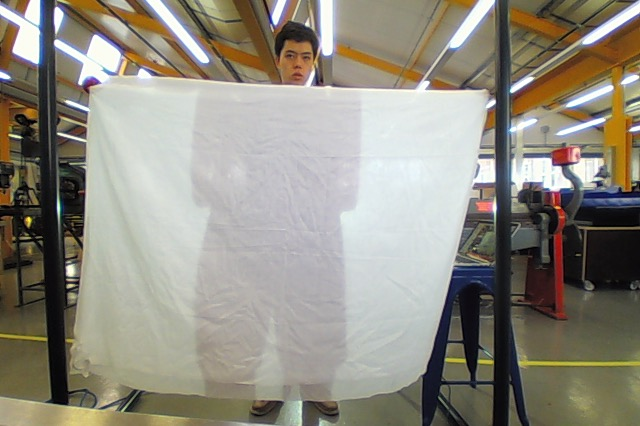
\includegraphics[width=0.5\textwidth]{figures/two_folds.jpg}
    \caption{... two layers seems to block a lot of the ambient background lighting}
  \label{fig:f2}
\end{figure}
\begin{figure}[H]
  \centering
    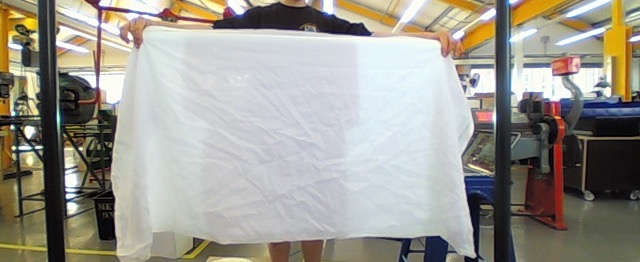
\includegraphics[width=0.5\textwidth]{figures/three_folds.jpg}
    \caption{... three layers blocks out too much of the intended lighting as well.}
  \label{fig:f2}
\end{figure}

Two folds seems to give the optimal clarity so I've purchased another 2mx1.5m peice of fabric.
Another problem that has turned up is that it is difficult to get the shadow of the feet to show up on the shadow screen. 
It seems like to fix this we'd need another light source at a lower height, but then we'd get two shadows which isn't really a very good idea.
I think at this point it seems like a wiser idea to restrict the reconstruction from the waist up (ideally we'd have a large raised platform and a parabolic light reflector, but time, skill and monetary constraints render this infeasible).

In other news, there's been progress on the turntable. 
The cogs have been cut out. 
It only remains to 3D print the smaller cog, to lubricate the bearings, get the motor working and then put together the circuit.

\begin{figure}[H]
  \centering
    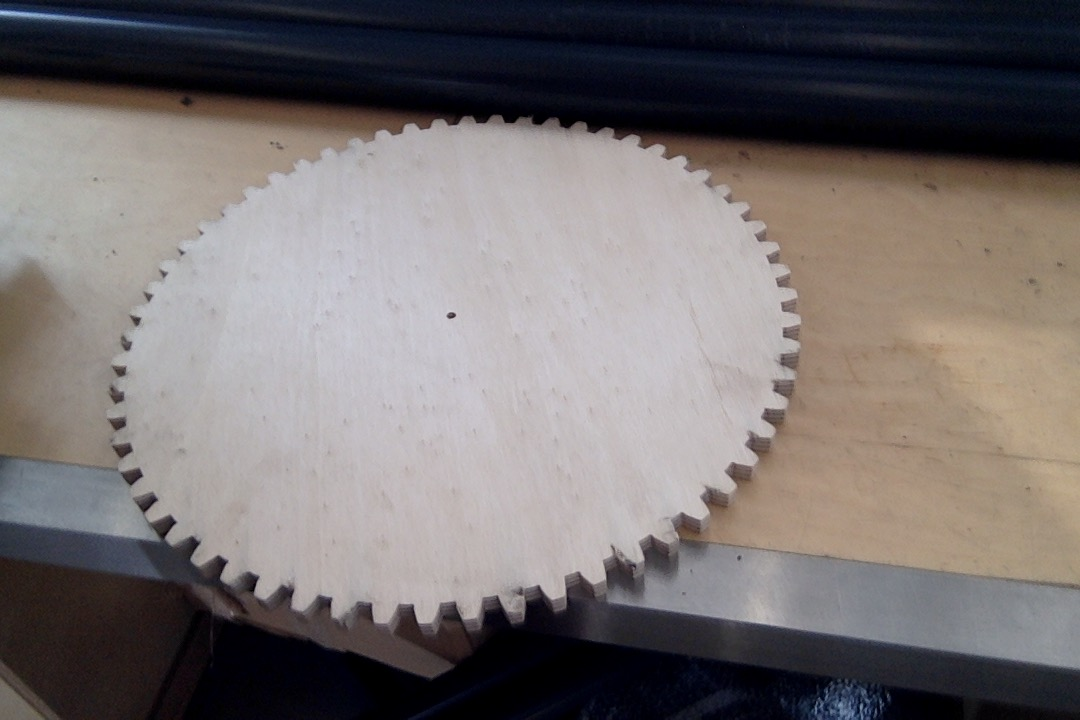
\includegraphics[width=0.7\textwidth]{figures/cog.jpg}
    \caption{The turntable cog.}
  \label{fig:f2}
\end{figure}

\section{Week 8}

\subsection{Building}
\subsubsection{3D Printing}
Finally a lot of the building came together this week.
The week started with 3D printing the smaller cog and its mount.

\begin{figure}[H]
  \centering
    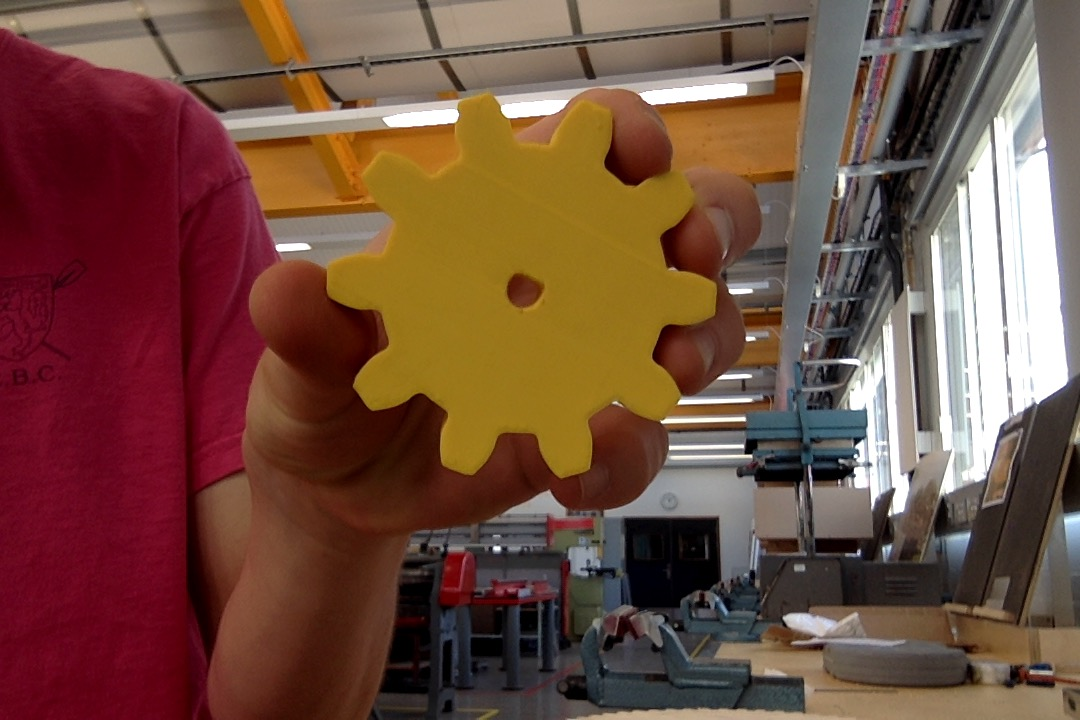
\includegraphics[width=0.7\textwidth]{figures/printed_cog.jpg}
    \caption{3D printed cog}
  \label{fig:f2}
\end{figure}

I got the design of the cog from the website which outlines how to create a turntable.
This was the first time I'd 3D printed something and it was an interesting experience.
The file with the cog design had to be converted to an appropriate file format for the 3D printer using an archaic Chinese conversion software!
Anyway, with that out of the way I proceeded to print the cog in roughly 5h.

Once that was done I tried inserting the motor shaft, but it turned out that the hole was too small so I had to use a file to widen it.
The problem with this however was that the plastic material used wasn't too strong so when we tested the turntable later on, the hole got damaged and so the shaft just spun in its spot while the cog did not turn.
The timing for this was particularly inopportune (the day before the final demonstration) so I had to come up with a quick solution.
Thanks to the advice of Dr. Roebuck, I cut out a thin metal sheet, carefully bent the sheet into a cylinder with a flattened side and inserted it into the cog for reinforcement. 
This luckily enough, did fix the problem (although I had to spend a lot of extra time filing the hole again).

I then needed to print the mount.
This was a particularly instructive if not slightly punishing learning experience.

\begin{figure}[H]
  \centering
    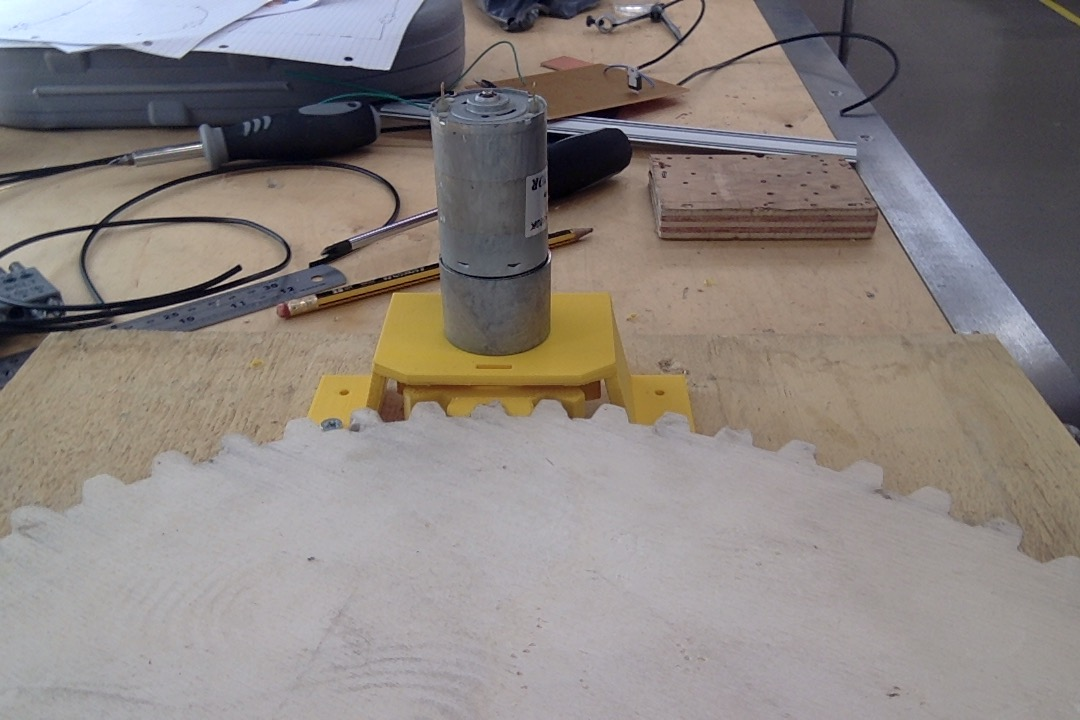
\includegraphics[width=0.7\textwidth]{figures/mounted_motor.jpg}
    \caption{Mount, motor and cog}
  \label{fig:f2}
\end{figure}

You can see the mount below the motor in the picture above.
As you can see, it is hollow where the cog is supposed to go.
Well, on this day I learned that 3D printers cannot print over thin air!
To print the mount the 3D printer needed to also print a support below the suspended part of the mount. 
I thought this meant some sparsely spaced pillars, but it turned out it printed a solid block of 3D plastic which I had to manually remove with pliers and a file.
Consequently the mount took 8h (!) to print.
A much smarter thing to have done would have been to print the mount on its side.
This would probably have halved the printing time and saved probably over half the printing material!

\subsubsection{Circuits and souldering}
While these parts were printing I mostly worked on the circuitry.
It is worth noting I have never touched a souldering iron in my life before this and so it was quite the learning curve.
Dr. Roebuck kindly helped with the circuit design and pointed out a fatal mistake I had made in my design (I had connedted the MOSFET the wrong way around).
He also instructed me in how to soulder.
As it turns out, souldering is more of an art than anything else.
My first soulders were abysmal failures that just burnt the wires and didn't actually do anything.
The biggest challenge was to hold the wire in place while also holding the souldering metal and the souldering iron all the same time.
Luckily the Dyson center had one of these contraptions to help with extra hands:

\begin{figure}[H]
  \centering
    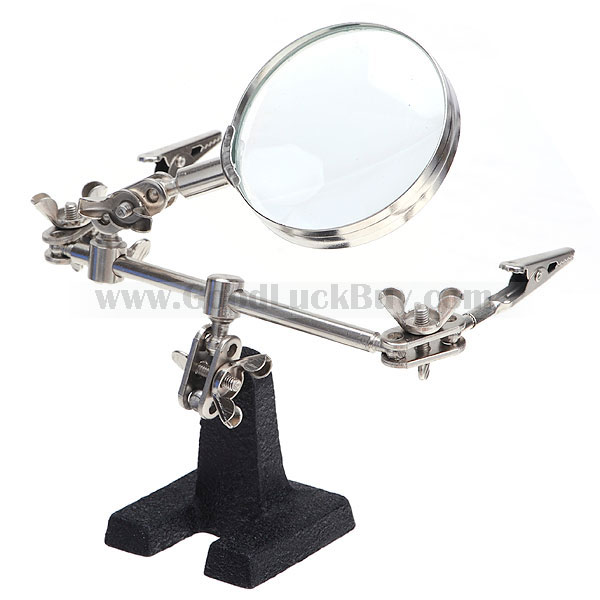
\includegraphics[width=0.7\textwidth]{figures/clamps.jpg}
    \caption{An extra pair of hands (image from www.goodluckbuy.com).}
  \label{fig:f2}
\end{figure}

The other tricky part was attaching the power cables to the circuit.
Unlike the other wires, these were thicker and so could not be inserted into the holes in the strip board.
They had to first be saturated with soulder and then melted again to attach to the underside of the board.
Having never souldered before it took roughly 4-5 frustrating attempts before I even came close to attaching anything.
Even when it was attached, it turned out there were still gaps between the wire and the copper strip and so another 2-3 attempts ensued.
You can see my first rather poor attempt highlighted in the red rectangle.

\begin{figure}[H]
  \centering
    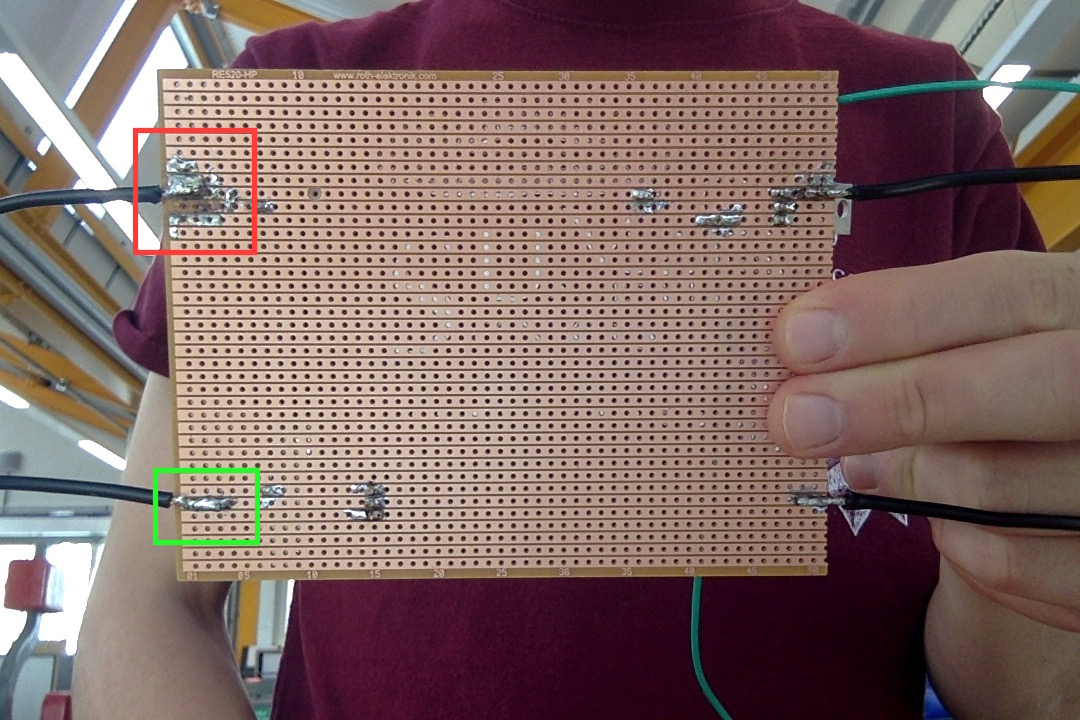
\includegraphics[width=0.7\textwidth]{figures/circuit_1_red.jpg}
    \caption{Evidence that I managed to soulder a circuit (poorly)}
  \label{fig:f2}
\end{figure}

In theory the soulder should only have been on one of the copper strips. 
However as you can see I did not have to skill to manage that on my first attempt and I consequently nearly short circuited the whole attempt.
To fix this I had to use a soulder sucker by melting the soulder between the copper tracks and then sucking up the soulder.
The green rectangle is how the whole mess should've looked like.
Note however that the green rectangle was Dr. Roebuck demonstrating how to attach the power cords so I'm afraid I cannot take credit for that one.

I cannot complain though. Learning to soulder and work with circuits was definitely the highlight of this project for me.

\subsubsection{Assembly}
With most of the parts now made, it remained to piece it all together.
The motor got screwed onto the mount and the mount got screwed to the base.
The large cog was attached to the bearing by drilling large holes in the base so that it the cog could be screwed on.
Then the motor needed to be souldered to the circuit and the circuit needed to be attached to the base.
To do this part I got 8 bolts and 4 screws, drilled holes into the corners of the circuit board and then placed 2 bolts below each hole, before drilling it to the base.
This prevented the circuitry from directly touching the base which could potentially cause damage.
Lastly I needed to soulder the parallel port adapter to the circuit so that the turntable could be connected to a computer.
This was actually a non trivial task as I needed to make sure that the correct pins were connected at the right points so that everything could be controlled smoothly from the comfort of my computer terminal (mostly though, it was non trivial because I am still bad at souldering).

\begin{figure}[H]
  \centering
    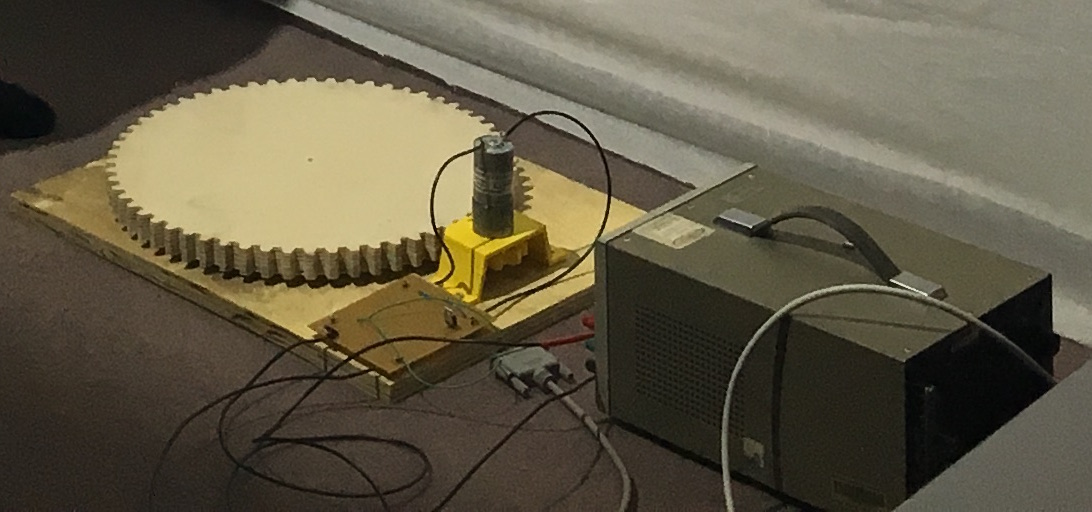
\includegraphics[width=0.7\textwidth]{figures/assembly.jpg}
    \caption{Final assembly}
  \label{fig:f2}
\end{figure}

I also purchased the second layer of fabric for the back drop and sewed on elastic cloth bands so that the fabric could be attached to the frame.

\begin{figure}[H]
  \centering
    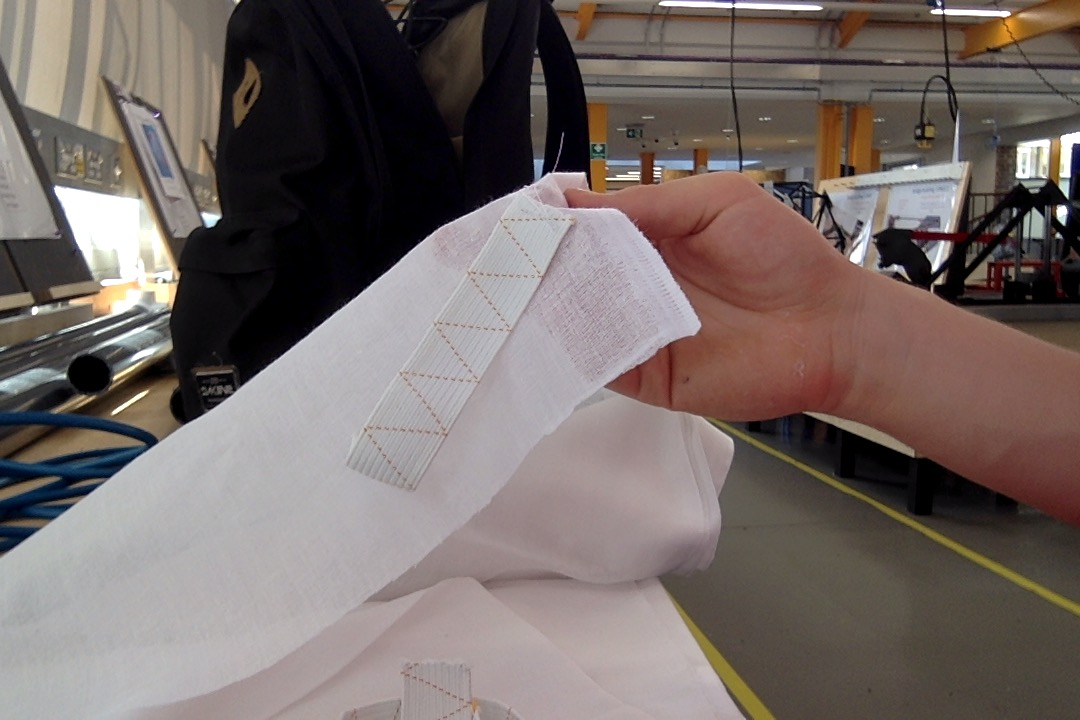
\includegraphics[width=0.7\textwidth]{figures/sewing.jpg}
    \caption{Sewing on elastic cloth bands.}
  \label{fig:f2}
\end{figure}

\subsubsection{Reamining tasks: Electronics and power supply}
There were a few things that I didn't manage to finish in time for the demonstration.
First of all I didn't have access to a computer with a parallel port at the engineering department so I had to improvise by using a manual square wave generator to fake the output a computer would generate.

I also didn't have time to finish the part of the circuit with the micro switch.
The purpose of this was so that we'd know exactly how many teeth had passed when each picture was taken so that we could calculate the angle that the cog had turned.
Without this part of the circuit I had to hack together rather poor timer based approach that estimated the angle by estimating the time elapsed.
The problem with this approach is that actually taking the picture takes a non negligible amount of time to do and so the estimate is not great.

\begin{figure}[H]
  \centering
    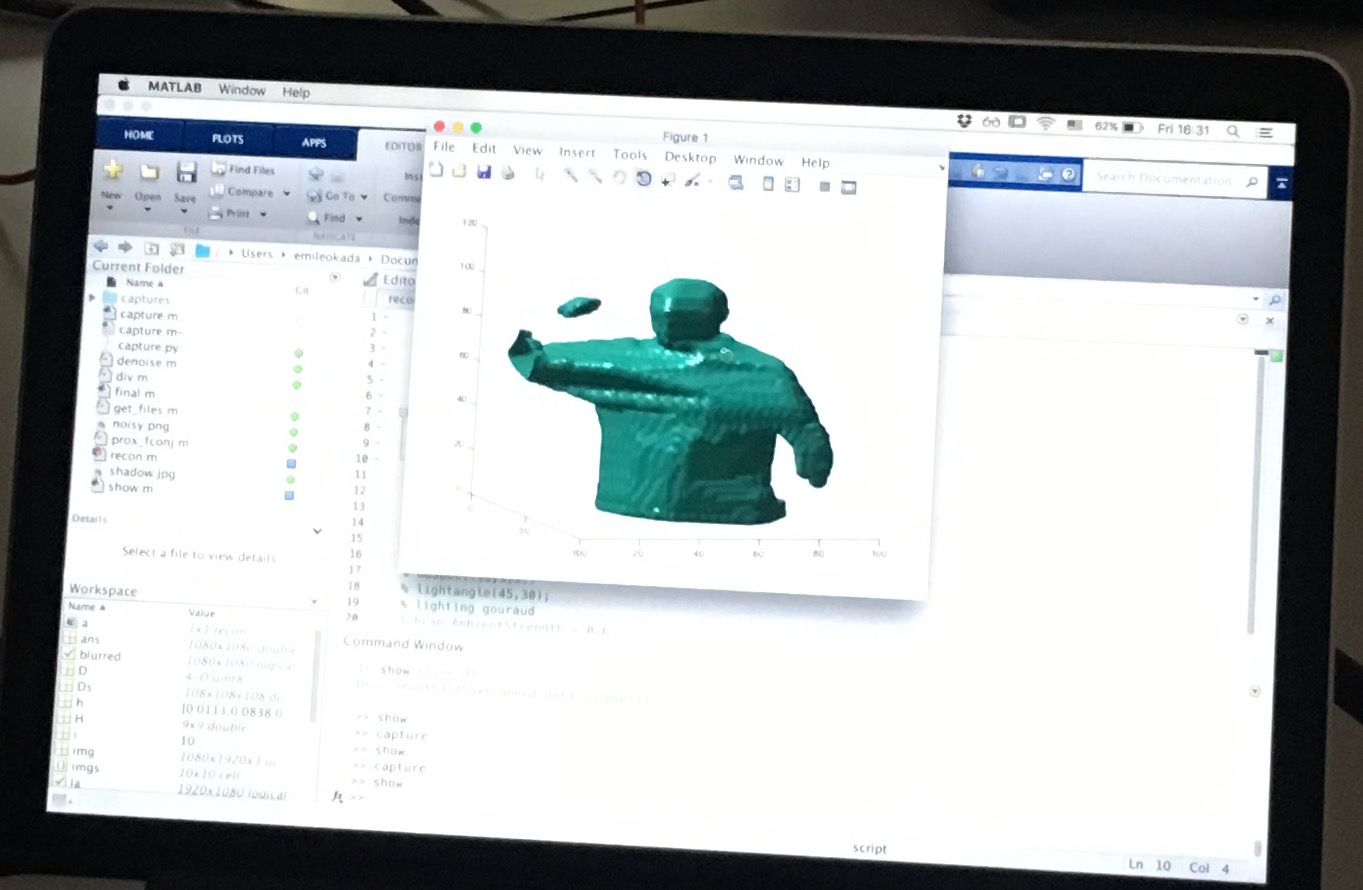
\includegraphics[width=0.7\textwidth]{figures/martin_recon.jpg}
    \caption{Martin striking a striking pose.}
  \label{fig:f2}
\end{figure}

What that meant is that not only did the reconstruction become distorted, but in fact, thin objects like arms might disappear altogether!

I'd quite like to fix this part of the circuit before the science fair in Easter.

Lastly, I need to get a more nimble power supply. 
The reason why the 15kg behemoth variable current and voltage power supply was used was to figure out how much current was required to drive the motor.
Now that that has been sorted I can easily get a nice and simple cable.

\subsection{Code}
The only remainig thing I need to do here is get a hold of a computer with a parallel port and then code up the interface.
Also, in the end I decided to not use the TV transform for smoothing and instead go with Gaussian smoothing with a small kernel for the sake of speed.

\newpage
\section{Code}
\subsection{3D reconstruction from shadows}
\label{alg:shadow}
\lstinputlisting[language=Python]{../recon/recon.m}
\end{document}

